\documentclass{article}
\usepackage[utf8]{inputenc}
\usepackage{graphicx}

\title{Geometrical Algorithms}
\author{Taein Kim, Utkarsh Goyal}
\date{May 2021}

\begin{document}

\maketitle

\section{Introduction}

Geometrical Algorithms are algorithms that deal with with distance, area, and other geometrical components in a 2D or 3D plane. The input is usually the location of some given points and lines, which you will have to write code to calculate the result.

\section{Sum of Manhattan Distances Between a Set of Points}

This is a simple but prime example of a geometrical algorithm problem. The Manhattan distance between two points is the sum of their x- and y-coordinate differences. Given a set of points, you want to find the sum of every Manhattan distance between every pair.

\subsection{The Naive Approach}

The easiest approach to go about this problem is using a nested loop to recurse through every pair of points. Although this is simple, it runs in $O(n^2)$ time and is inefficient. Here is an example:

\begin{figure}[htp]
    \centering
    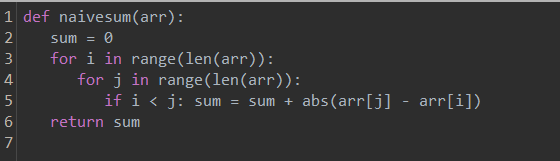
\includegraphics{NaiveSum.png}
    \caption{The Naive Code}
\end{figure}

\subsection{The Efficient Approach}

For us to run the same program in $O(N \log N)$ time, we need to realize what adding one point to an existing array does to the algorithm. We simply have to add the sum of every distance from the new point. Thus, with a sorted array, 
\[newsum = oldsum + \sum{(x_i-x)} = oldsum + x_i * i - \sum{x}\]
This is implemented in code:

\begin{figure}[htp]
    \centering
    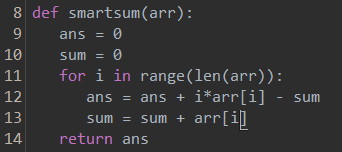
\includegraphics{SmartSum.png}
    \caption{The Efficient Code}
\end{figure}

\section{Klee's Algorithm}

Given an array of segments on a line, is there a way to find the length of the union of segments?
Hint: you'll have to find a way to subtract the overlaps from the total length of the segments (Greedy Algorithm?) Try to make it run in O(N log N) time.

\subsection{Explanation}

Obviously in a union, the order of the coordinates does not matter; you can just store every coordinate in a vector array, indicating whether the coordinate is a starting point or endpoint. After that, sort the array and traverse; keep count of the number of "open" sections, making sure that you reach 0 at the end. Otherwise, only add the difference between the previous and current points to your sum when there are open lines traversing the current section.

\section{Divide and Conquer}
The divide and conquer algorithm works exactly as the name suggests; you divide and then you conquer. This may sound really simple at first, but this algorithm is used a lot in problems involving geometric algorithms. One very common example is finding the closest pair of points in O($n$ log $n^2$). 
\subsection{Naive Approach}
Naive Approach: As many of you probably know, you can just go through each possible pair of points and just find the maximum distance. However, this takes $O(n^2)$ time.
\begin{figure}[htp]
    \centering
    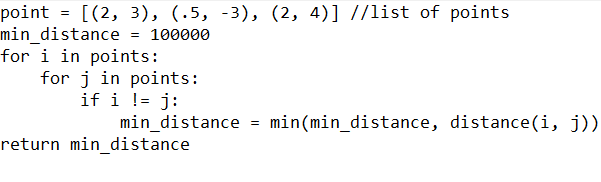
\includegraphics{NaiveDistance.png}
    \caption{Naive Code to find minimum distance between two points}
\end{figure}
\subsection{Divide and Conquer Approach}
    \begin{figure}
    \centering
    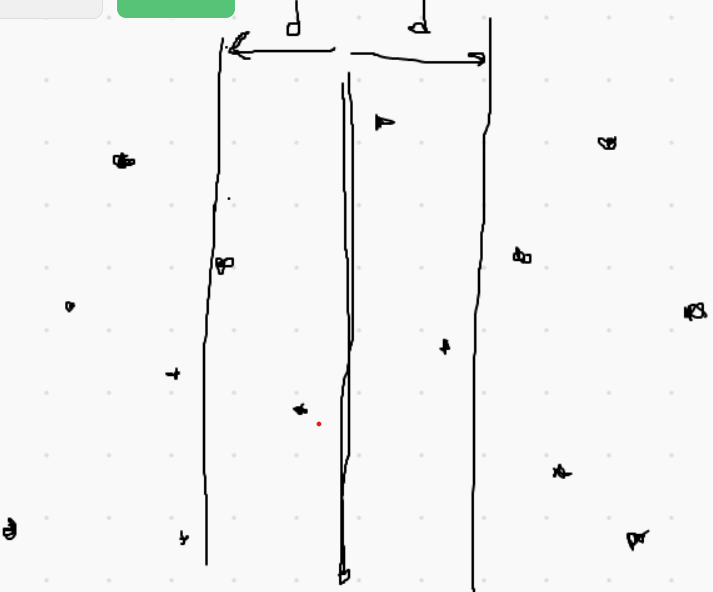
\includegraphics[scale=.5]{distance.png}
    \caption{Reference for step 4 in divide and conquer algorithm}
    \end{figure}
Here are the following steps:

\begin{enumerate}
    \item Sort the array with respect to the x-coordinates(it doesn't really matter if you were to sort with respect to y-coordinates)
    \item Split the array into two halves, from $0 - n/2$ and $(n/2 + 1) - (n - 1)$
    \item Recursively find the smallest distances between points from each of the array, and then find the minimum of the two distances you get. Let's call this value $d.$
    \item Now, since we haven't accounted for the distance of points that are in both strips, we realize that we only have to consider the ones that are $d$ away from the middle point. This is because if the distance from the middle is greater than $d$, then it won't have a smaller distance than the distance we've already gotten.(Reference Figure 4)
    \item We can sort all the points from step 4 by y-coordinate(O(n log n)); its worth mention that this can be optimized to O(n) if you use merge sort. 
    \item From here, we find the smallest distance in this sorted set of points.
    \item We finally just return the minimum of d and the value from the previous step.
\end{enumerate}
\subsection{Further Explanation of Step 6 and Time Complexity}
For step 6, even though this may seem like $O(n^2)$ time complexity, we can actually make it $O(n)$ as its sorted. In reality, we actually just have to check $7$ points after the current one. (I'll leave proving this as an exercise to the reader.) To find the overall time complexity of a recursive algorithm like this, we can mark the complexity as $T(n).$ Then, with dividing the array into two arrays of reduced length, $T(n/2)$, and finding and sorting the strip of coordinates by y-coordinates in O($n$ log $n$ + $n$), and finding the minimum distance in the strip in $O(n)$, we have $T(n) = T(n/2) + O(n\log{n} + n) + O(n).$ Simplifying this, we get $T(n) = T(n (\log{n})^2).$

\section{Challenge Problem}
Given a set of points on the 2D plane, how could we find the maximum number of them that lie on the same line?

\end{document}

